\documentclass[../main.text]{report}
\subsection{Code: Création d'ensembles aléatoires}
Les codes des appendices \ref{code:generate_set_p} et \ref{code:generate_odd_set_p} sont ceux utilisés pour générer les ensembles aléatoires par algorithme probabiliste. Ceux-ci possèdent des complications inutiles, dues au fait que nous enregistrions au départ les ensembles sous forme de tableau de données. Nous montrons ces algorithmes tels quels, car ce sont ceux qui ont été utilisés pour générer les ensembles. Nous proposons cependant en appendice \ref{code:simplified_generator} une version simplifiée de code. 


\subsubsection{Création d'ensembles probabiliste}
\label{code:generate_set_p}
Le code suivant génère 100 ensembles aléatoires non-impairs. 
\lstinputlisting[language=R]{../r_code/generate_samples2.R}

\clearpage
\label{code:generate_odd_set_p}
\subsubsection{Création d'ensembles probabiliste impairs}
\lstinputlisting[language=R]{../r_code/odd_prob_sets.R}

\clearpage
\label{code:simplified_generator}
\subsubsection{Création d'ensembles probabiliste impairs}
\lstinputlisting[language=R]{../r_code/simplified_generator.R}

\subsubsection{Création d'ensembles par l'approche analytique}
\label{code:approche_analytique}
Le code qui suit comprend toutes les fonctions utilisées pour créer les ensembles aléatoires via l'approche analytique, les manipuler et tracer tous les graphes de la section \ref{sec:analytique}.
\lstinputlisting[language=Python]{../py_code/approche_analytique.py}

\clearpage
\subsection{Seconde conjecture} 
\label{code:conj_2_3_report}
\subsubsection{Rapport de conjecture}
Le code suivant génère un tableau de donnée pour chaque ensemble, contenant le nombre d'entiers vérifiant la conjecture, le nombre d'échec et le plus grand entier ne vérifiant pas la conjecture.
\lstinputlisting[language=Python]{../py_code/conjecture_2_3.py}

\clearpage
\subsection{Test conjecture}
Le code suivant vérifie l'assertion pour tout entier, après avoir donné fourni les limites supérieures et inférieures. Aucun rapport n'est généré, mais le programme échoue dès qu'un entier ne satisfait pas les conditions de l'assertion
\lstinputlisting[language=Python]{../py_code/test_conj_2_3.py}

\clearpage
\subsubsection{Error mapping}
\label{code:Error_mapping}
\lstinputlisting[language=Python]{../py_code/conjecture2_3_error_mapping.py}

\subsection{Code pour le test de la conjecture \ref{conj:twinprimes}}
\lstinputlisting[language=Python]{../py_code/conjecture.py}

\subsection{Graphes supplémentaires}

\begin{figure}[H]
 \centering
 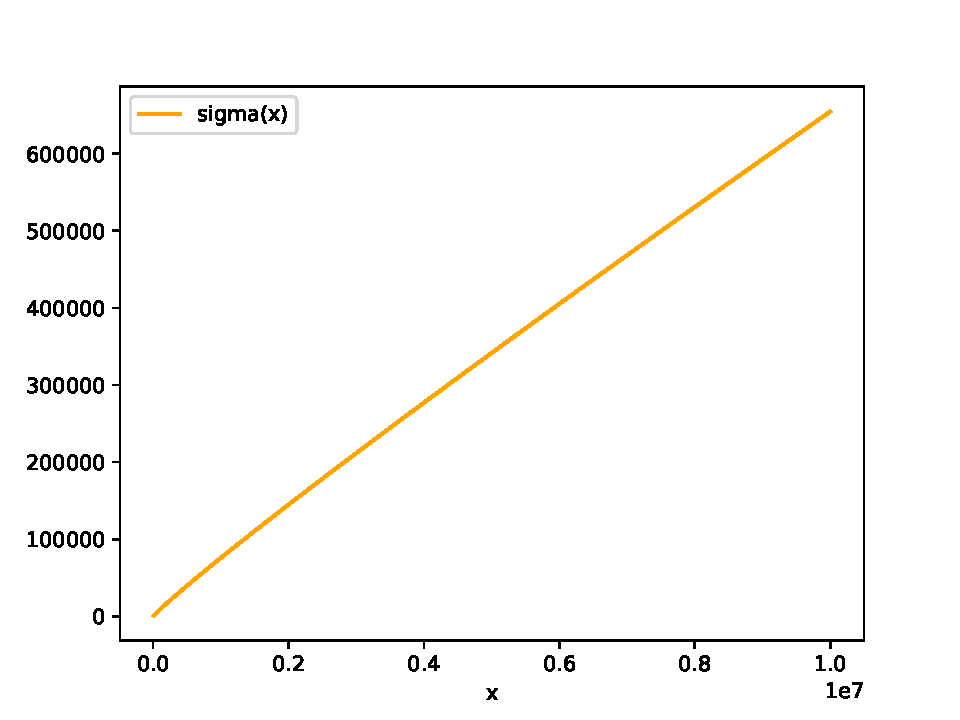
\includegraphics[keepaspectratio=true, width=12cm]{analytic_sets.pdf}
 \caption{Graphe de $\sigma_{Q}$ pour tous les ensembles $Q$ }
 \label{im:image212}
\end{figure}

\begin{figure}[H]
 \centering
 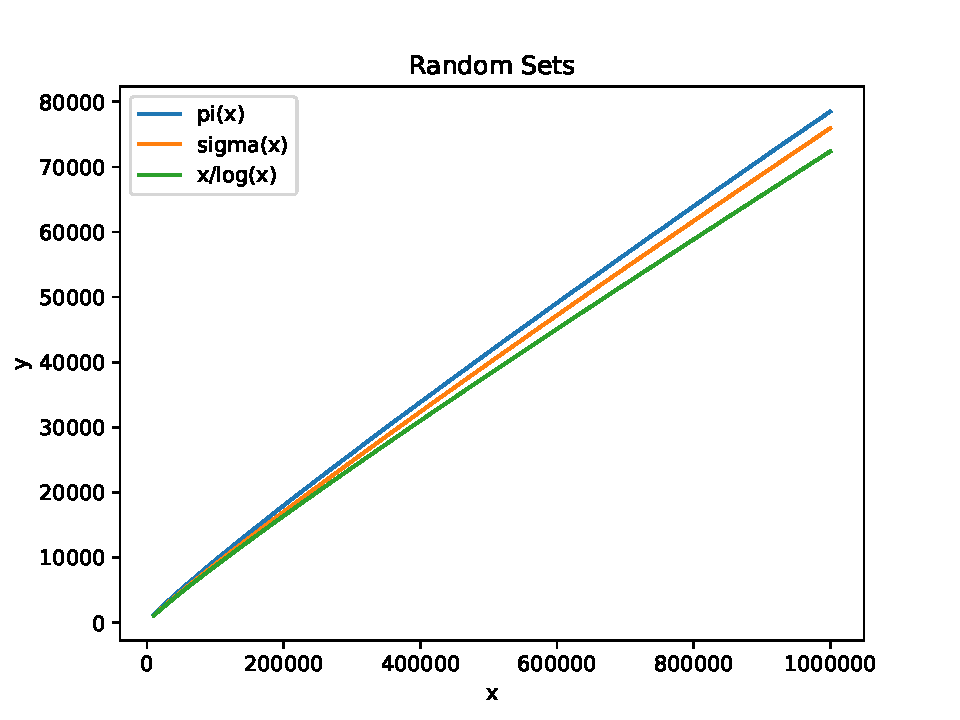
\includegraphics[keepaspectratio=true, width=12cm]{analytic_approach_sets_1.pdf}
 \caption{Figure \ref{im:image1} pour $x$ jusqu'à $10^4$ }
 \label{im:image2131}
\end{figure}

\begin{figure}[H]
 \centering
 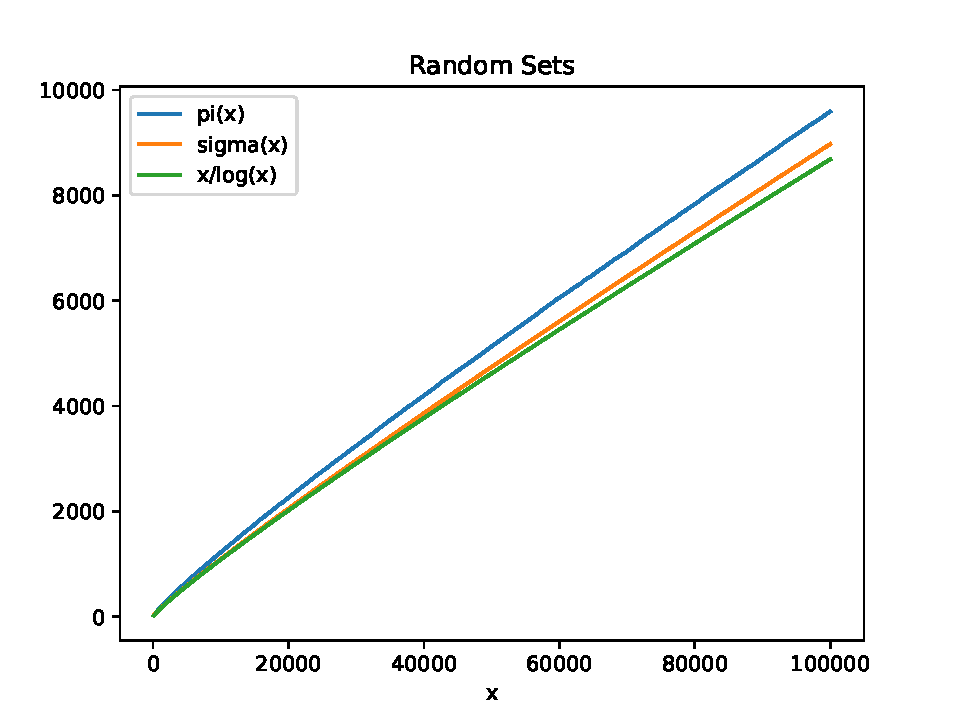
\includegraphics[keepaspectratio=true, width=12cm]{analytic_approach_sets_2.pdf}
 \caption{Figure \ref{im:image1} pour $x$ jusqu'à $10^5$ }
 \label{im:image2132}
\end{figure}

\begin{figure}[H]
 \centering
 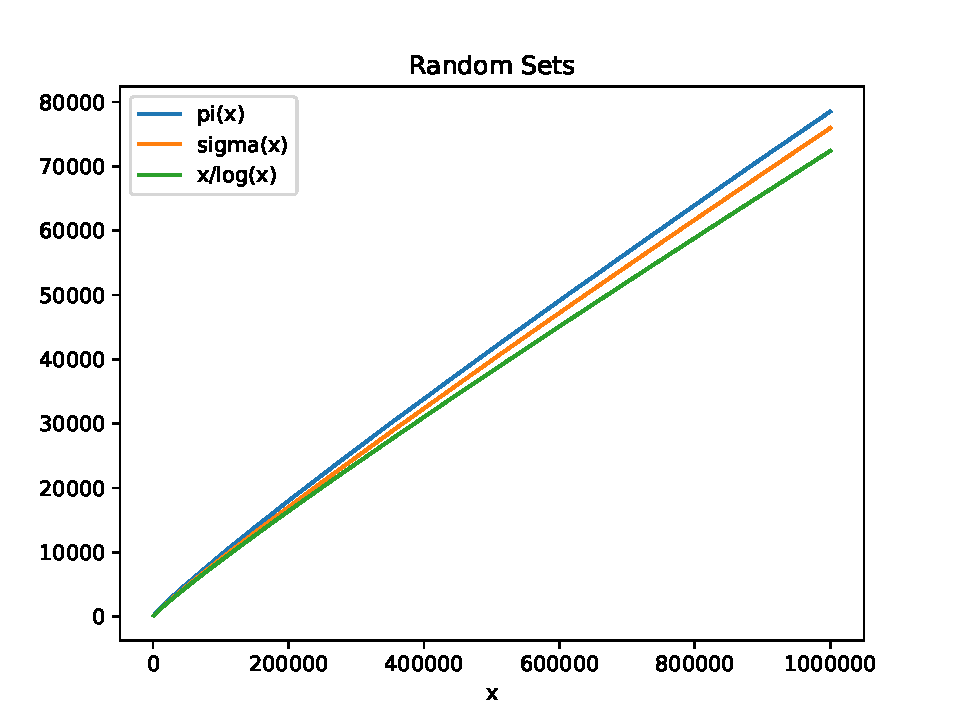
\includegraphics[keepaspectratio=true, width=12cm]{analytic_approach_sets_3.pdf}
 \caption{Figure \ref{im:image1} pour $x$ jusqu'à $10^6$ }
 \label{im:image2133}
\end{figure}
